% this file is called up by thesis.tex
% content in this file will be fed into the main document
\ifpdf
    \graphicspath{{figures/}{figures/comparisons}}
\else
    \graphicspath{{figures/}{figures/comparisons}}
\fi

\chapter{Reconstruction using Sensor Fusion rotation and 3-point translation}
As previously shown using sensors for camera translation estimation give quite big errors, resulting in especially poor epipolar line matching. This especially prevents one from getting highly accurate results in dense matching (which strongly relay on epipolar line calculation) and from getting highly detailed 3D models. \\
Because of that author in his research had an idea to combine traditional image based methods for translation estimation with Sensor Fusion approach for camera rotation. Following chapter describes his deliberations on that approach as well as evaluation performed for verification.
\section{Concept}
From section 9.2 of Multiple View Geometry \cite{HartleyMultipleView} it is known that
\begin{equation} \label{eq:relativeFundamntal}
\textbf{x}_{'}^{T}\textbf{F}\textbf{x} = 0
\end{equation}
and also that for relative camera based system ($P = \begin{bmatrix}I |0\end{bmatrix}, P' = \begin{bmatrix}R|t\end{bmatrix}$) fundamental matrix can be written as:
\begin{equation} \label{eq:relativeFundamntal}
\textbf{F} = \textbf{K}^{-T}\begin{bmatrix}\textbf{T}\end{bmatrix}_{x}\textbf{R}\textbf{K}^{-1}
\end{equation}
where 
\begin{equation} \label{eq:skewTranslation}
\begin{bmatrix}\textbf{T}\end{bmatrix}_{x} = 
\begin{bmatrix*}[c]
 0 & -t_{z} & t_{y}\\
 t_{z} & 0 & -t_{x}\\
-t_{y} & t_{x} & 0 
\end{bmatrix*} 
\text{where \textbf{T}} = \begin{bmatrix}t_{x},t_{y},t_{z}\end{bmatrix}
\end{equation}
By combing two above equations, it can be rewritten as:
\begin{equation} \label{eq:relativeFundamntal}
\textbf{x}_{'}^{T}\textbf{K}^{-T}\begin{bmatrix}\textbf{T}\end{bmatrix}_{x}\textbf{R}\textbf{K}^{-1}\textbf{x} = 0
\end{equation}
And finally as:
\begin{equation} \label{eq:alternative3point}
\textbf{x}_{'}^{T}\textbf{K}^{-T}\begin{bmatrix*}[c]
 0 & -t_{z} & t_{y}\\
 t_{z} & 0 & -t_{x}\\
-t_{y} & t_{x} & 0 
\end{bmatrix*}\textbf{R}\textbf{K}^{-1}\textbf{x} = 0
\end{equation}
Having:
\begin{equation} \label{eq:leftRelative}
\begin{array}{lcl}
\textbf{h}_{'}^{T} &=& \textbf{x}_{'}^{T}\textbf{K}^{-T} \\
\textbf{h} &=& \textbf{R}\textbf{K}^{-1}\textbf{x} \\
\end{array}
\end{equation}
and substituting those values in \ref{eq:alternative3point}:
\begin{equation} \label{eq:alternative3point}
\begin{bmatrix*}[c]
h_{'1} & h_{'2} & h_{'3}
\end{bmatrix*}\begin{bmatrix*}[c]
 0 & -t_{z} & t_{y}\\
 t_{z} & 0 & -t_{x}\\
-t_{y} & t_{x} & 0 
\end{bmatrix*}\begin{bmatrix*}[c]
h_{1} \\
h_{2} \\
h_{3}
\end{bmatrix*}
= 0
\end{equation}
When multiplying it one receives the following:
\begin{equation} \label{eq:alternative3point}
h_{1}\cdot h_{'2}\cdot t_{z} - h_{1}\cdot h_{'3}\cdot t_{y} - h_{2}\cdot h_{'1}\cdot t_{z} + h_{2}\cdot h_{'3}\cdot t_{x} + h_{3}\cdot h_{'1}\cdot t_{y} - h_{3}\cdot h_{'2}\cdot t_{x}
= 0
\end{equation}
which can be grouped:
\begin{equation}
t_{x} \cdot  (h_{2}\cdot h_{'3} - h_{3}\cdot h_{'2}) + t_{y} \cdot  (h_{3}\cdot h_{'1} - h_{1}\cdot h_{'3}) + t_{z} \cdot  (h_{1}\cdot h_{'2} - h_{2}\cdot h_{'1}) = 0
\end{equation}
and rewritten as:
\begin{equation} \label{eq:translation3point}
\begin{bmatrix*}[c]
t_{x} &
t_{y} &
t_{z}
\end{bmatrix*}\begin{bmatrix*}[c]
(h_{2}\cdot h_{'3} - h_{3}\cdot h_{'2}) \\ 
(h_{3}\cdot h_{'1} - h_{1}\cdot h_{'3}) \\
(h_{1}\cdot h_{'2} - h_{2}\cdot h_{'1}) 
\end{bmatrix*} 
= 0
\end{equation}
then solved for instance with SVD with only three points pairs, because the equation has only 3 unknown variables (translation in three axes). However, in such situation the overall accuracy strictly depends on the precise measurements of camera rotation, because value of \textbf{h} depends on it. Thus every error in rotation estimation will influence also translation estimation using proposed 3-point method.
%: ----------------------- name of chapter  -------------------------
\section{Implementation} % top level followed by section, subsection
When it is known or assumed that the acquired rotation data is accurate, the translation can be calculated with the 3-point algorithm. The proposed equation \ref{eq:translation3point} was implemented in a way similar to other fundamental matrix estimations methods implemented in OpenCV. This particular implementation also has the ability to properly filter outliers with the use of RANSAC algorithm and its listing, written in self-documenting style, can be seen below:
\begin{lstlisting}
    ...
    for (iterationNumber = 0; iterationNumber < niters; iterationNumber++) {

        getSubsety(prev_points_raw, next_points_raw, point1s, point2s, 300, modelPoints);
        Mat t = findTranslation(point1s, point2s, rotDiffGlobal, Kinv);
        Mat F1 = constructFundamentalMatrix(rotDiffGlobal, t, Kinv);

        int goodCount = findInliersy(prev_points_raw, next_points_raw, F1, errors, statuses, reprojThreshold);
        if (goodCount > maxGoodCount) {
            swap(statuses, goodStatuses);
            FEnhanced = F1;
            tEnhanced = t / t.at<double>(2);
            maxGoodCount = goodCount;
            niters = cvRANSACUpdateNumIters(confidence,
                    (double) (count - maxGoodCount) / count, modelPoints, niters);
        }

    }
    ...    
    
    Mat findTranslation(std::vector<cv::Point2d> &points1, std::vector<cv::Point2d> &points2, Mat &rotDiff, Mat &Kinv) {

    Mat hg1 = Mat::zeros(points1.size(), 3, CV_64FC1);
    Mat hg2 = Mat::zeros(points2.size(), 3, CV_64FC1);
    for (int i = 0; i < points1.size(); i++) {
        hg1.at<double>(i, 0) = points1[i].x;
        hg1.at<double>(i, 1) = points1[i].y;
        hg1.at<double>(i, 2) = 1;
        hg2.at<double>(i, 0) = points2[i].x;
        hg2.at<double>(i, 1) = points2[i].y;
        hg2.at<double>(i, 2) = 1;
    }

    hg1 = hg1 \cdot  (rotDiff \cdot  Kinv).t();
    hg2 = hg2 \cdot  (Kinv).t();

    Mat A = Mat::zeros(hg1.rows, 3, CV_64FC1);
    for (int i = 0; i < hg1.rows; i++) {
        A.at<double>(i, 0) = (hg2.at<double>(i, 2) \cdot  hg1.at<double>(i, 1) - hg2.at<double>(i, 1) \cdot  hg1.at<double>(i, 2));
        A.at<double>(i, 1) = (hg2.at<double>(i, 0) \cdot  hg1.at<double>(i, 2) - hg2.at<double>(i, 2) \cdot  hg1.at<double>(i, 0));
        A.at<double>(i, 2) = (hg2.at<double>(i, 1) \cdot  hg1.at<double>(i, 0) - hg2.at<double>(i, 0) \cdot  hg1.at<double>(i, 1));
    }

    SVD svd1(A);
    Mat tCalc = svd1.vt.row(2);

    //Translation between cameras estimated and Fundamental Matrix from that as well
    Mat T = (tCalc.t());

    return T;

\end{lstlisting}

\section{Evaluation}
In case of this approach previously conducted translation accuracy tests do not have much comparison. Currently calculated translation doesn't have realistic global scale, because there isn't anything it could be referenced to. The only thing that can be evaluated is whether epipolar line calculations are more accurate than in Sensor Fusion based approach. \\
In figures \ref{fig:f_01_3point} and \ref{fig:f_02_3point} are presented the epipolar lines calculated from Fundamental matrices constructed from translation estimated using proposed 3-point approach and rotation from sensors. It's good to compare them with epipolar lines visualised in figures \ref{fig:f_01_sensor} and \ref{fig:f_02_sensor}. They are much more accurate keeping the condition of crossing the corresponding matches. Evaluation of time efficiency and numerical accuracy are conducted in Chapter \ref{sec:Testin2Views}. \\
At this point of his research, author had an idea to try another approach, which could produce quite even better effects - usage of Sensor Fusion rotation data in standard 5-point and 8-point algorithms for \textbf{F} calculation. This would allow on both image based translation estimation and possibly correction of sensor influenced rotation error matrix estimation. 
\begin{figure}[h!]
    \centering
    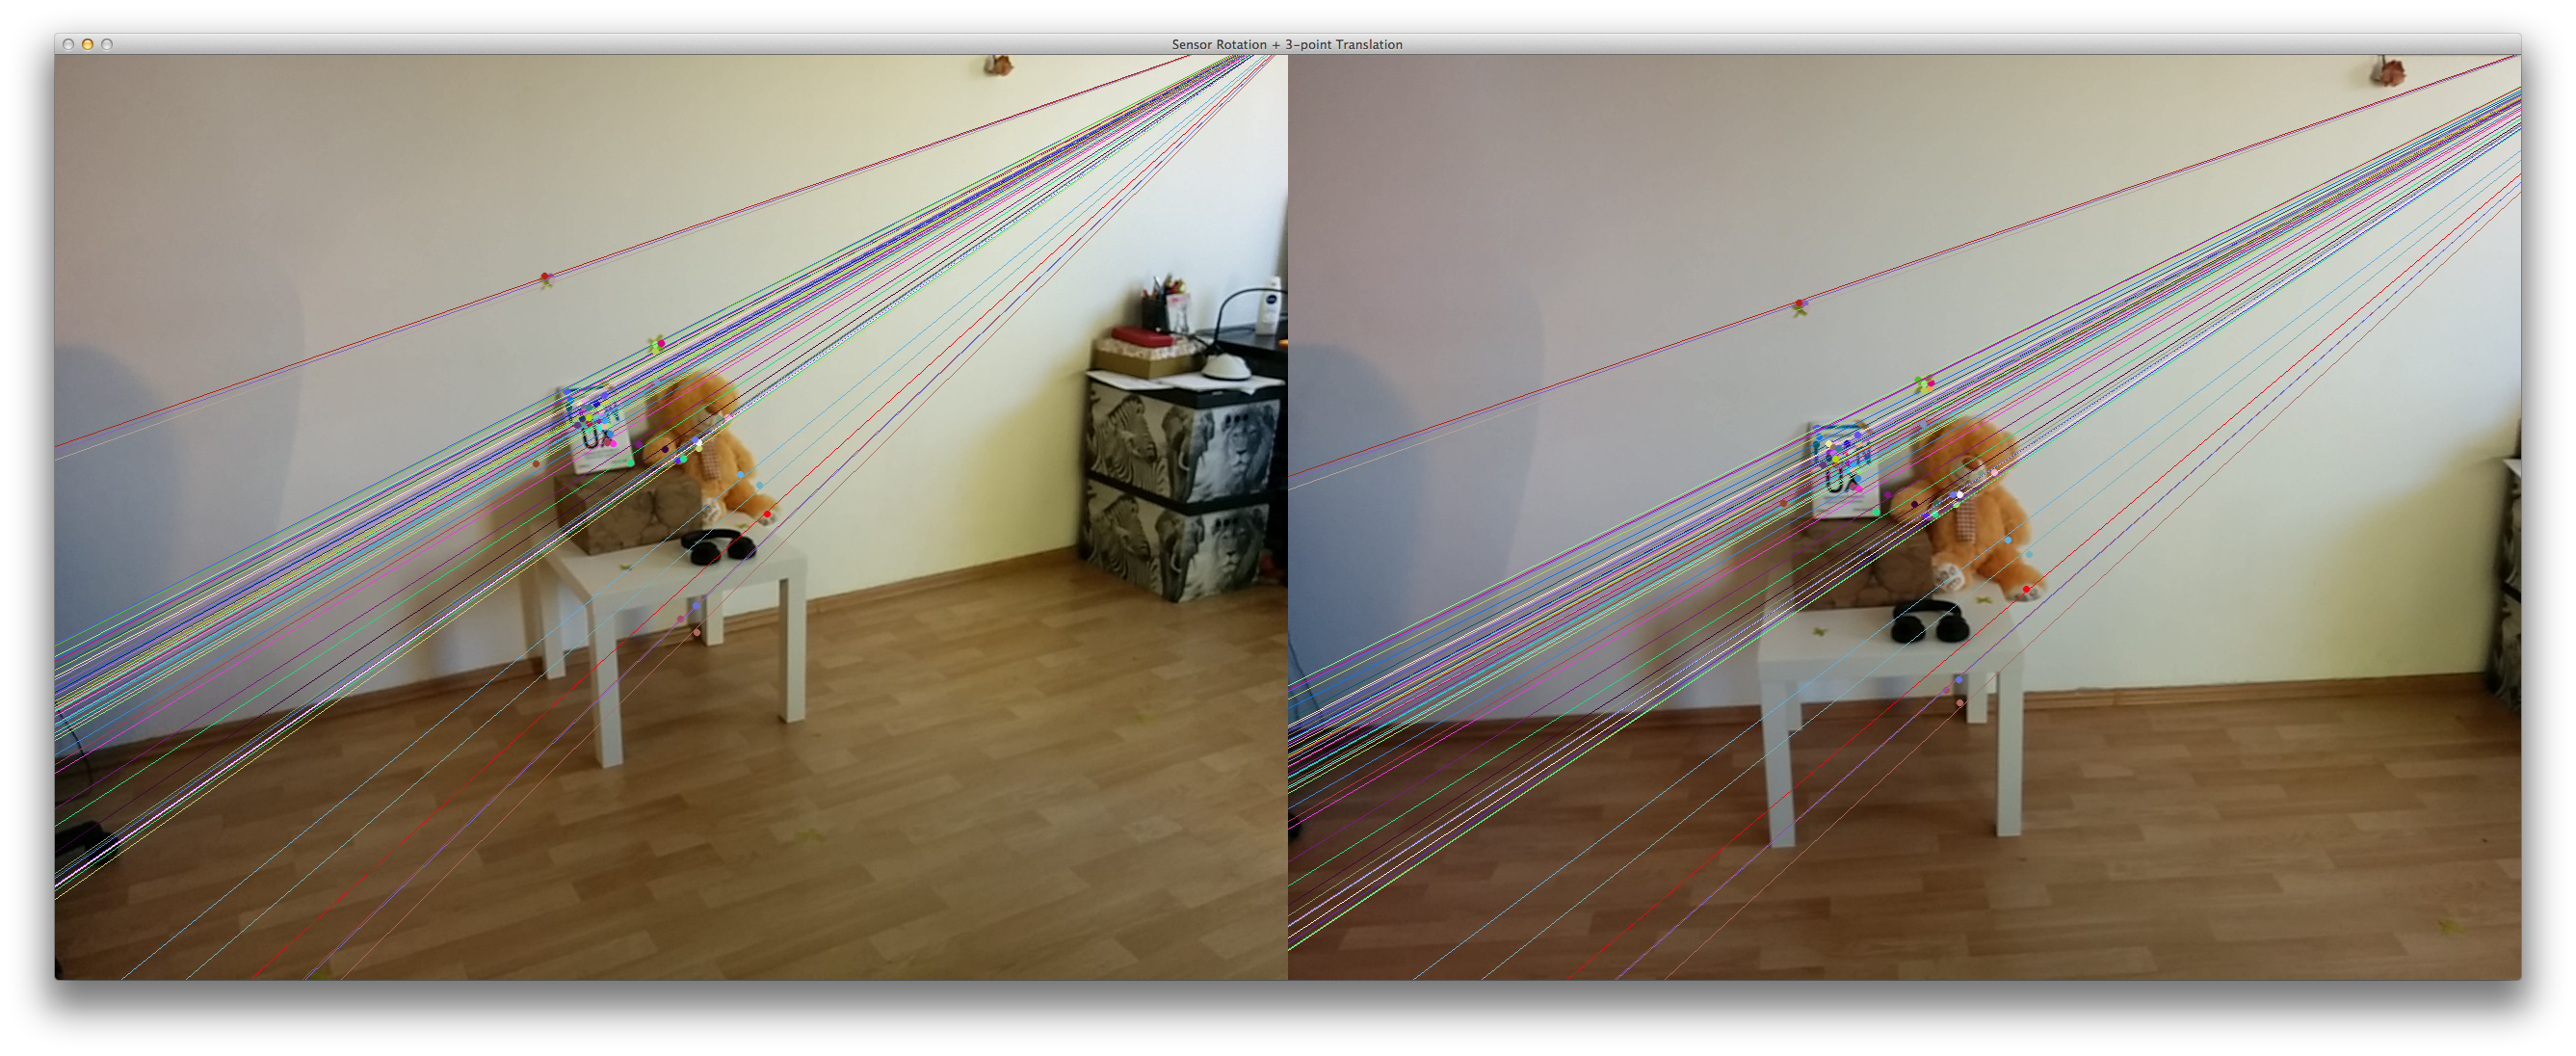
\includegraphics[width=0.8\textwidth]{f_01_3point}
    \caption[Visualisation of epipolar lines for 3-point translation estimation and Sensor Fusion rotation approach - 1st example]{Visualisation of epipolar lines for 3-point translation estimation and Sensor Fusion rotation approach for images 0.jpg and 1.jpg in test dataset. It can be seen that in comparison to \ref{fig:f_01_sensor} epipolar lines cross or at least are close to corresponding points.}
    \label{fig:f_01_3point}
\end{figure}

\begin{figure}[h!]
    \centering
    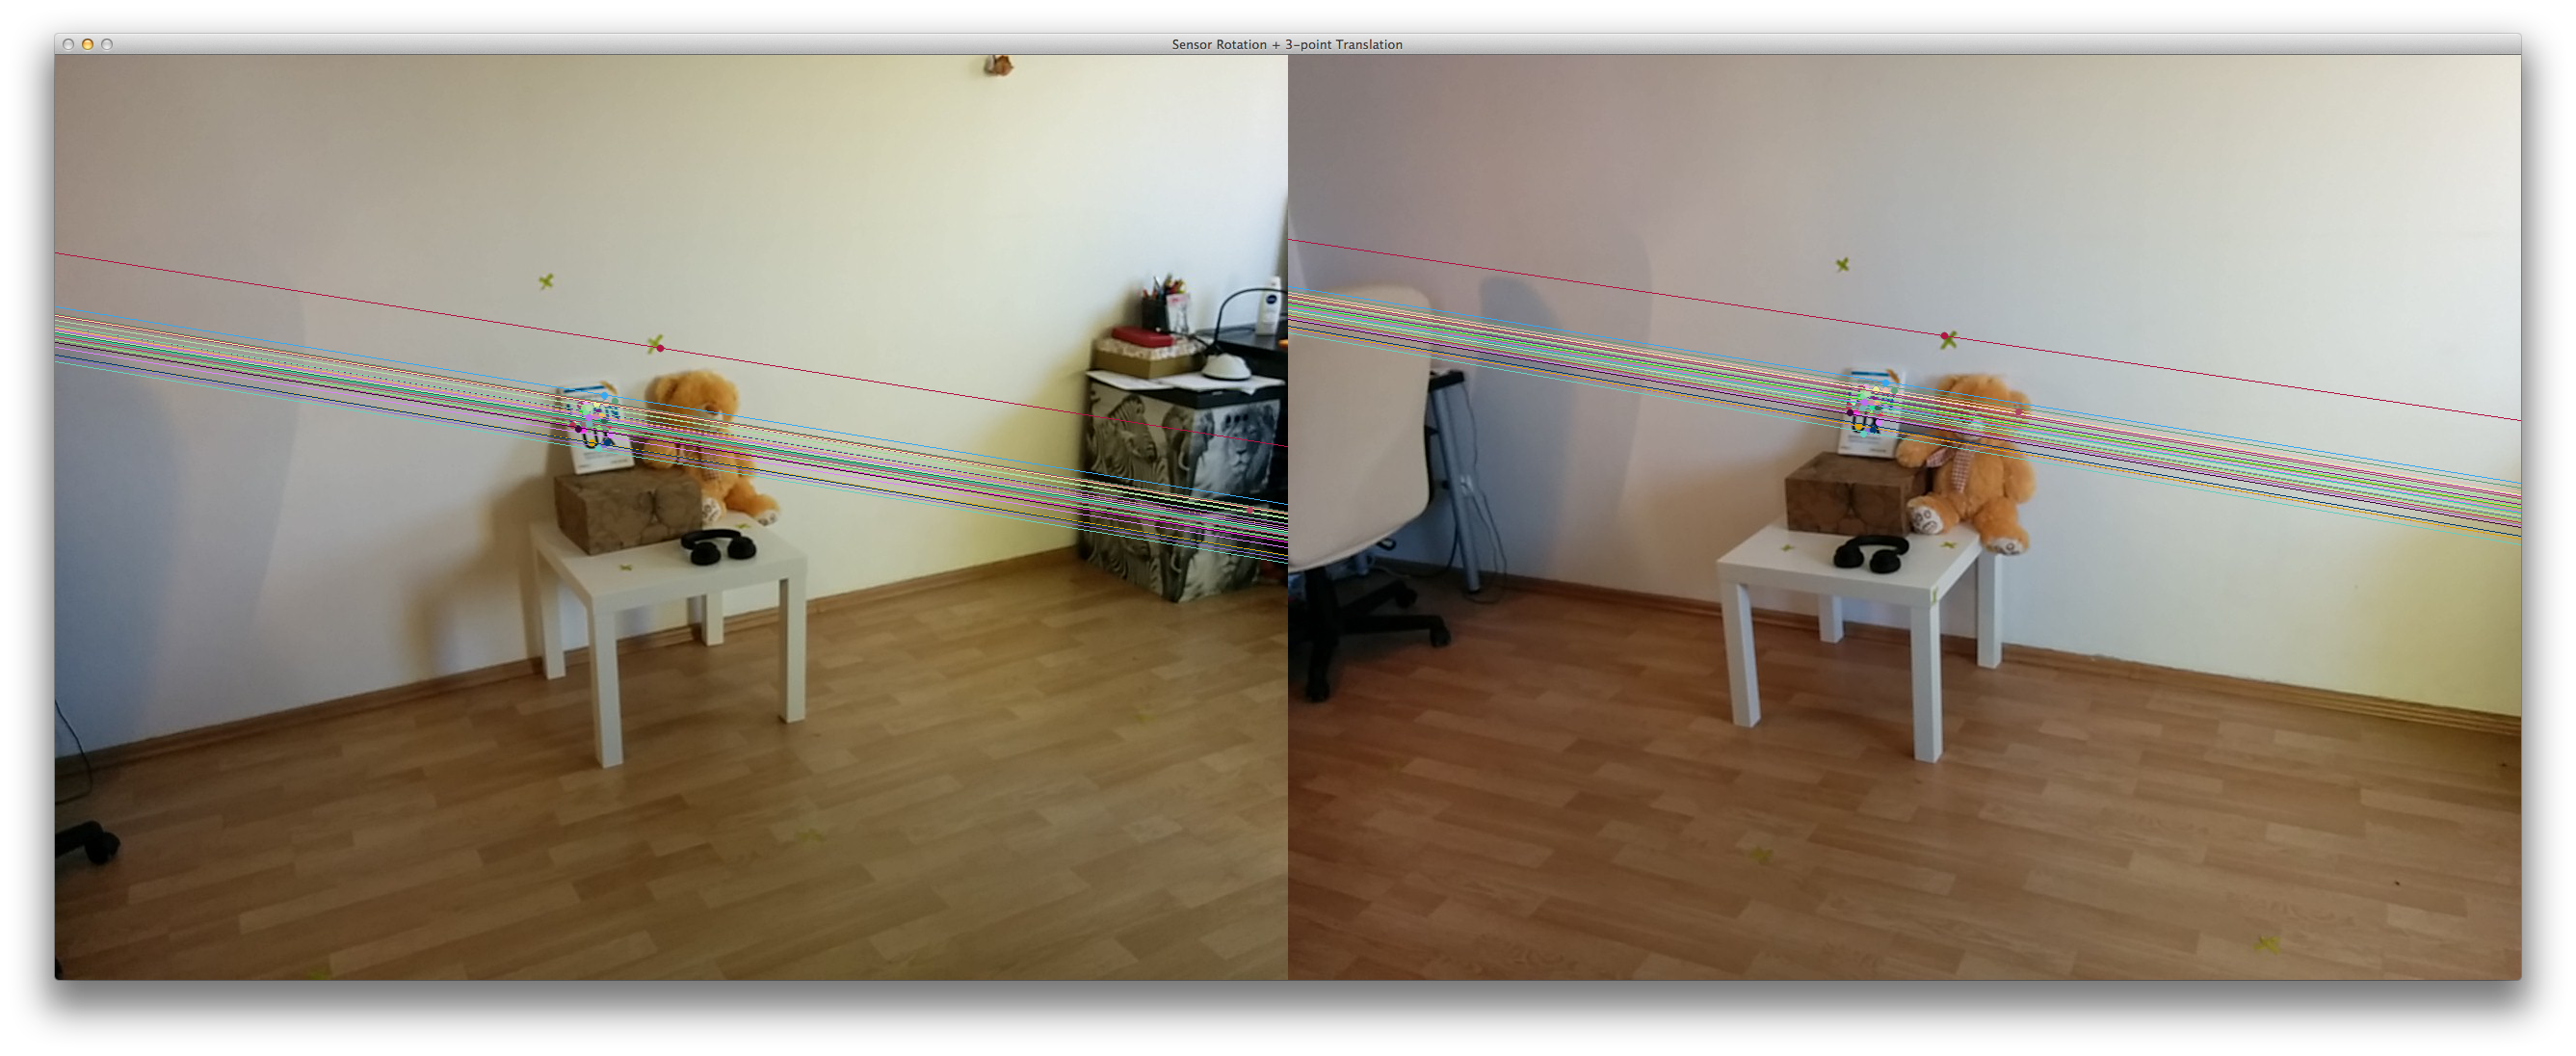
\includegraphics[width=0.8\textwidth]{f_02_3point}
    \caption[Visualisation of epipolar lines for 3-point translation estimation and Sensor Fusion rotation approach - 2nd example]{Visualisation of epipolar lines for 3-point translation estimation and Sensor Fusion rotation approach for images 0.jpg and 2.jpg in test dataset. It can be seen that in comparison to \ref{fig:f_02_sensor} epipolar lines cross or at least are close to corresponding points.}
    \label{fig:f_02_3point}
\end{figure}



% ---------------------------------------------------------------------------
% ----------------------- end of thesis sub-document ------------------------
% ---------------------------------------------------------------------------
